\providecommand{\main}{./report}
\documentclass[../main.tex]{subfiles}
\begin{document}


\section{Experiments}\label{section:experiments}
Accompanying the proposal of a new feature- ranking and selection methodology, there is an experiment. The aim of the experiment is to show an example of what is possible with both the pipeline, and the newly proposed evaluation methodology. In this way, \gls{ml} practitioners and authors of new methods are able to conduct experiments themselves with the same setup and configuration: therefore allowing comparison between the experiments.



\subsection{Experiment setup}
The experiment closely follows the outlines of Section~\ref{section:evaluation} and Section~\ref{section:pipeline}. The setup can be summarized like so:

\begin{itemize}
    \item The dataset at hand is split into a 80\% training- and 20\% testing dataset. Whereas the training set is reserved for fitting the feature ranker and validator, the testing set is reserved for scoring the validator.
    \item For each Feature Ranker and dataset, $B = 25$ bootstrap resampling iterations are run.
    \item In each bootstrap resampling iteration, $\min (p, 50)$ feature subsets are evaluated, with each including the $k$ best features.
    \item Validation estimators are evaluated with the R\textsuperscript{2} score in case of regression and with accuracy in the case of classification. The validation estimators used are \gls{knn} with $k=5$ and a \gls{dt} at default sklearn settings.
    \item In the aggregation process, in case several experimental runs are found with the same configuration, i.e., for one Feature Ranker executed on one dataset, only the `best' run is considered. The best run is considered to be the run with the highest average mean score over all features, considering all bootstraps. This aggregation step will be elaborated upon in Section~\ref{section:experiments-example}.
\end{itemize}

All experiments were run on a SLURM \gls{hpc} environment. Specifically, the University of Groningen has a `Peregrine' compute cluster, with machines of various types, of which the most common one is a 24 core machine powered by two Intel Xeon E5 2680v3 CPUs running at 2.5 GHz. Per node, 128 GB memory and 1 TB internal disk space is available, but 10 GB was requested per CPU instead. This accounts for a total of 100 GB memory for 10 CPU processes. In total, the experimentation facilitating these results took 7682 hours of processing time on the above-mentioned machines.


A line-up of feature rankers and datasets was constructed to conduct benchmarking on. The full list of both is available in the Appendix Section~\ref{section:appendix-experiment-lineup}. See Table~\ref{table:experiments-ranker-specification} for the Feature Ranking line-up, and Table~\ref{table:experiments-dataset-specification} for the datasets line-up. The distribution of classes can be found in Appendix Figure~\ref{fig:experiments-datasets-class-distributions}. Most datasets are balanced, though also some imbalanced ones are included. Imbalanced datasets are not treated specially, it is up to the ranking- and validation estimators to correct for this. It can also be seen that rankers of various types are included: both regressors and classifiers, and rankers that support both learning tasks. Furthermore, some rankers were included that support multioutput datasets, i.e., datasets with multivariate targets.




%%% SYNCLF HARD %%
\subsection{Experimental results for the `Synclf hard' dataset}\label{section:experiments-example}
To best understand the format of the experimental results and the accompanying metrics, a look is taken at the results for one dataset. In this way, a better understanding of the charts is gained first.

% `Synclf hard`
First of all, the considered dataset is the `Synclf hard' dataset. It is a synthetically generated dataset, created using the sklearn \texttt{make\_classification} function (Section~\ref{section:pipeline-components-datasets}). Its full configuration specification is defined in Listing~\ref{code:pipeline-synthetic-example}. The dataset is defined to have $n=10000$ samples and $p=50$ dimensions. After the \gls{cv} step was conducted, 8000 samples are left for training. The dataset has 4 relevant features and 3 target classes, which are perfectly balanced. That said, observations are first made on running one feature ranker on the dataset. For this, ReliefF \citep{kononenko_estimating_1994} is chosen.
    



\subsubsection{ReliefF performance}

% All bootstraps validation performance
To start, a look is taken at a plot that explicitly plots \textbf{all bootstraps}. See Figure~\ref{fig:results-validation-dt-relieff}.

\begin{figure}[ht]
    \centering
    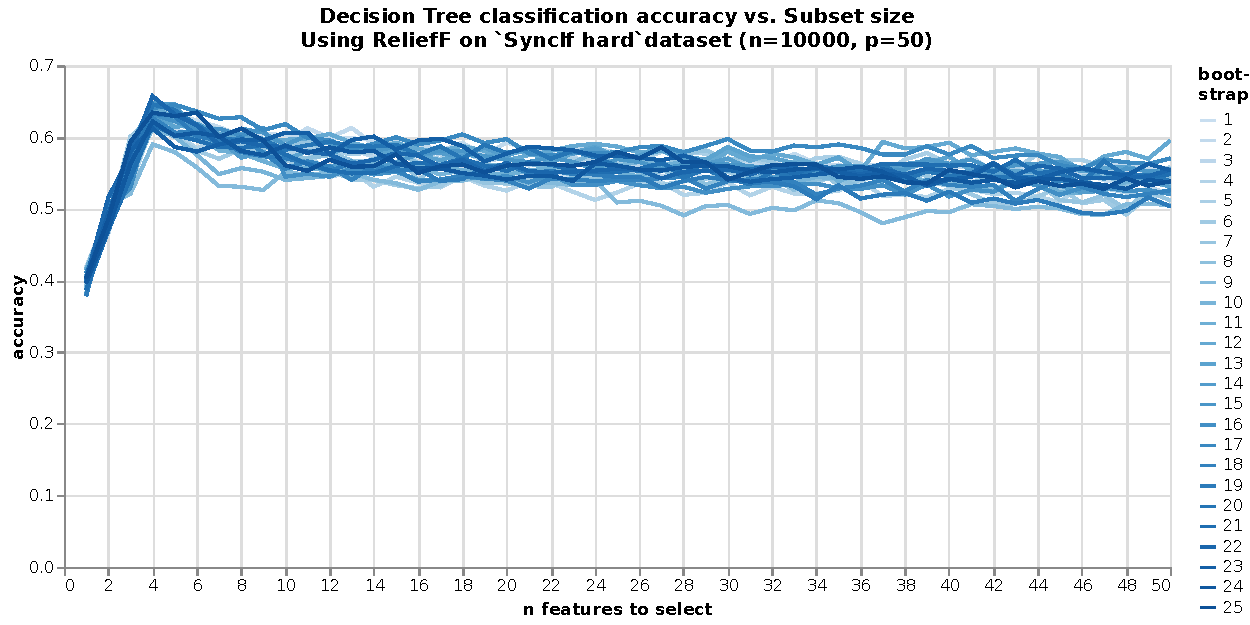
\includegraphics[width=\linewidth]{report/images/results-validation-dt-relieff.pdf}
    \caption{Validation performance for ReliefF on the `Synclf hard' dataset, for all 25 bootstraps.}
    \label{fig:results-validation-dt-relieff}
\end{figure}

As can be seen in Figure~\ref{fig:results-validation-dt-relieff}, the various bootstraps have had an effect on the validation performance per subset. Due to the random resampling with replacement taking place in the bootstrap phase, the feature ranker has to deal with permutations of the dataset each run. Indeed, this randomness is reflected in the validation performance.

One clear pattern is the fact that the validation performance first goes \textbf{up}, peaks at 4 features, and goes gradually down again. The fact that the peak happens at 4 features is clarified by the fact that the dataset had 4 informative features defined, meaning that the feature ranker correctly ranked the four informative features in its top-4 in most bootstraps. An intuition for the performance degradation is the fact that adding noisy dimensions can actually cause the estimator performance to degrade.



% Feature importance plot
Next, a better look is taken at the estimated \textbf{feature importances}. Since the validation performance suggests that the ranker correctly identifies the importance of the informative feature, it is expected that this is reflected in the feature importance estimates. Indeed, this is the case. See Figure~\ref{fig:results-importances-relieff}.

\begin{figure}[ht]
    \centering
    % 850x250
    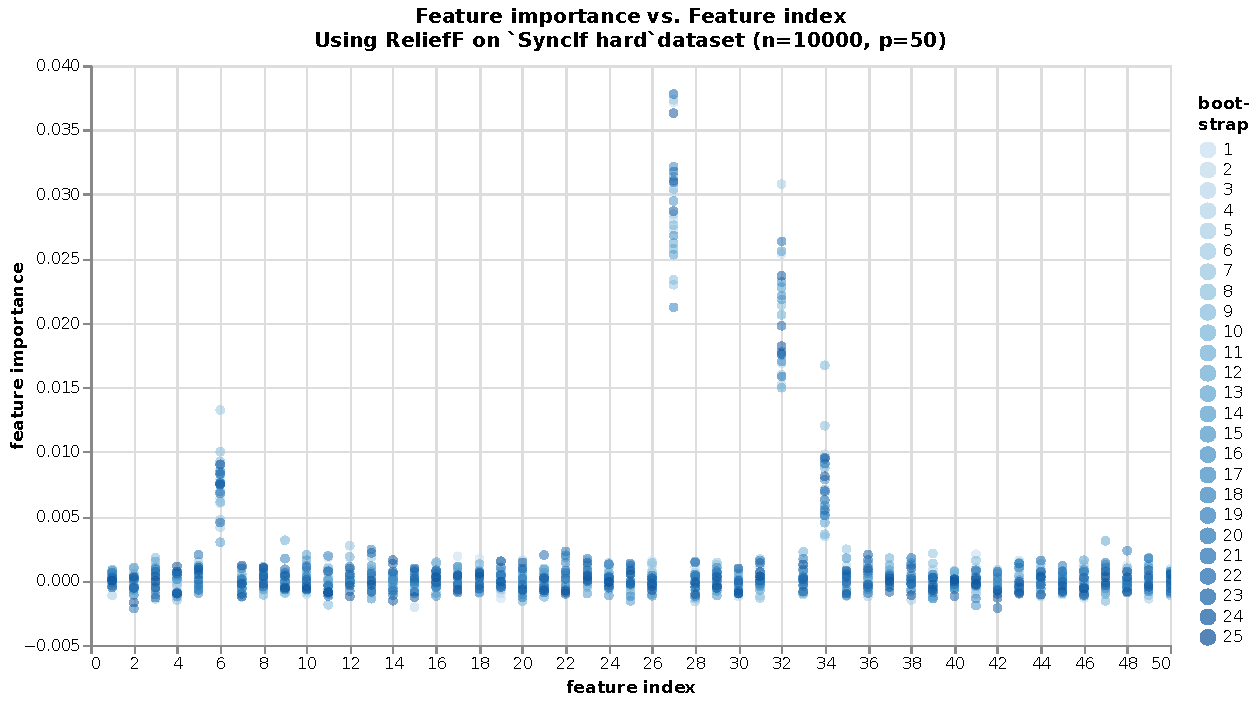
\includegraphics[width=\linewidth]{report/images/results-importances-relieff.pdf}
    \caption{Estimated feature importances for ReliefF on `Synclf hard'.}
    \label{fig:results-importances-relieff}
\end{figure}

It can be seen in Figure~\ref{fig:results-importances-relieff} that the first four features were assigned a larger importance than the others. Indeed, these are the ground-truth relevant features, as is known \gls{apriori} because the dataset was synthetically generated. Besides the `estimated' feature importances, also the \gls{gt} feature importance is visible. At all times, the \gls{gt} gets the same treatment as the estimated feature importances: it is also normalized to a probability vector. In this way, the two vectors can be compared fairly.

Using the information shown in Figure~\ref{fig:results-importances-relieff}, the R\textsuperscript{2} score and Log loss can now be computed between the estimated- and \gls{gt} feature importances. The computation is elaborated upon in Section~\ref{section:evaluation-apriori-knowledge}. The scores are shown in Table~\ref{table:experiments-relieff-gt-metrics}.

\renewcommand\theadalign{bl}
\begin{table}[ht]
    \centering
    \begin{tabular}{| l | l | l | l | l | l | l |}
    \hline
    \thead{Metric} & \thead{Mean} & \thead{Stdev} \\
    \hline
    R\textsuperscript{2} score & $0.6962$ & $\pm 0.0151$  \\ 
    \hline
    Log loss & $0.1749$ & $\pm 0.002517$\\ 
    \hline     
    \end{tabular}
    \caption{The R\textsuperscript{2}- and log loss metrics for ReliefF on `Synclf hard'. Scores were aggregated over 25 bootstraps, see Figure \ref{fig:results-importances-relieff}. Scores were computed like explained in Section~\ref{section:evaluation-apriori-knowledge}.}
    \label{table:experiments-relieff-gt-metrics}
\end{table}

The metrics in Table~\ref{table:experiments-relieff-gt-metrics} are to be interpreted as follows. In the case of the R\textsuperscript{2} score, a \textit{higher} score means a better result, i.e., means the ranker estimated the feature importances closer to the ground truth. The log loss, on the other hand, is desired to have a \textit{low} value; meaning the difference between the estimated- and the \gls{gt} importances were smaller. Next, lets see how to quantify the stability of the run.

To quantify the \textbf{stability} of estimated feature importance scores, the standard deviations of the feature importances are taken. First, the stdev score is computed for each feature over the $B$ bootstraps, and then the mean is taken over over the stdev scores. This is like it was explained in Section~\ref{section:feature-importance-stability}. The score can be plotted like it can be seen in Figure~\ref{fig:results-importances-stability-relieff-example}.

\begin{figure}[ht]
    \centering
    % 800x300
    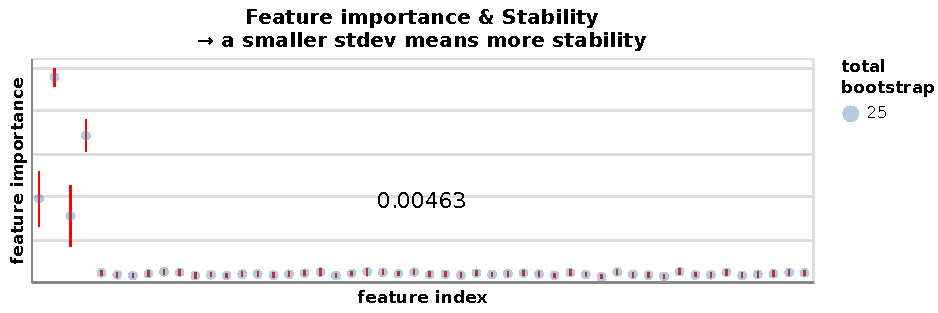
\includegraphics[width=0.9\linewidth]{report/images/results-importances-stability-relieff-example.pdf}
    \caption{Feature importance scores with stdev error bars and the total mean score visible. A higher stdev score means less stability. Shown for ReliefF on the `Synclf hard' dataset.}
    \label{fig:results-importances-stability-relieff-example}
\end{figure}

It can be seen in Figure~\ref{fig:results-importances-stability-relieff-example}, that the instabilities take place mainly in the relevant features. This means the algorithm is confident on which features \textit{not} to choose, but it is not sure about the weighting of the relevant ones. The mean stdev over all features is illustrated as text on the plot. Thanks to the red error bar lines, it can be quickly observed where the algorithm is instable. 

\subsubsection{Performance of multiple rankers}

% Combined validation performance chart
Next, multiple rankers are considered. Again, the dataset at hand is the `Synclf hard' dataset. The validation performance of all rankers can now be compared in a single plot, see Figure~\ref{fig:results-validation-dt-various-rankers}.

\begin{figure}[ht]
    \centering
    % 800x250
    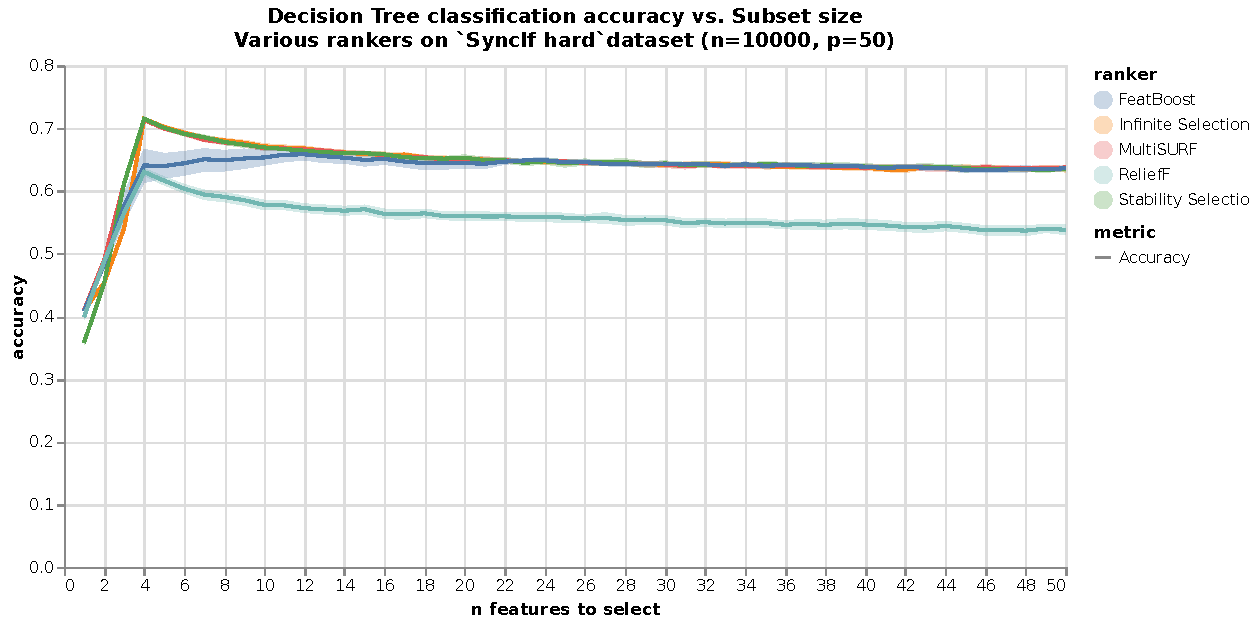
\includegraphics[width=\linewidth]{report/images/results-validation-dt-various-rankers.pdf}
    \caption{\gls{dt} validation performance of several rankers on the `Synclf hard' dataset.}
    \label{fig:results-validation-dt-various-rankers}
\end{figure}

In this case (Figure~\ref{fig:results-validation-dt-various-rankers}), the validation curve is \textbf{aggregated} over the bootstraps. That is, for each point on the curve, the average score is taken over the $B$ bootstraps. Looking at the plot, indeed, the various rankers show similar behavior like before in the validation performance. For most rankers, performance goes up, peaks at 4 features, and goes down again. Some rankers, however, do not manage to pick out the most useful features right away, and see their performance peak a bit later. It can also be the case that some rankers selected the most relevant features \textit{earlier} in their feature subsets, causing higher values at the start of the curve.



% Facet grid validation curve values
Another way to plot the validation curves is to put the curves side by side, instead of stacked upon each other. This allows illustrating an important aggregation metric: the \textbf{mean validation score}. As could be seen before, the validation curves are already assumed to be aggregated over the bootstraps. This means, the results for each ranker are now reduced to $\min(p, 50)$ values. To further reduce this value and be able to summarize the performance with a single \textit{scalar}, the mean of the aggregated validation curve is taken. See Figure~\ref{fig:results-validation-with-mean-score}.

\begin{figure}[ht]
    \centering
    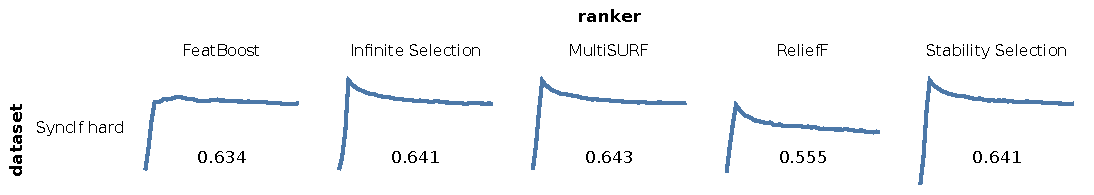
\includegraphics[width=\linewidth]{report/images/results-validation-with-mean-score.pdf}
    \caption{Aggregated \gls{dt} validation curves with their \textbf{mean validation score} shown. The mean score is the average curve value, allowing summarizing the curve with a single value. Curves are the same as in Figure~\ref{fig:results-validation-dt-various-rankers}.}
    \label{fig:results-validation-with-mean-score}
\end{figure}

Looking at the curves (Figure~\ref{fig:results-validation-with-mean-score}), it can be seen that the mean validation score scores higher where the curves scored a higher total score over all feature subsets. In this regard, the mean validation score could also be expressed as the sum of scores, or even the `area under the validation curve'. Because the tick steps on the x-axis are in this case always one, however, it is chosen to take the mean score instead. The detail lost by computing the interpolated curve pieces between the curve points is negligible. Taking the mean validation score is also a much easier metric to compute than the AUC, which in this case would require lots of interpolation. The mean validation score can be seen to represent the performance of the feature ranker reasonably well. When the ranker scores the relevant features as highly informative, the validation score appropriately reflects this. Feature rankers that have a low area under the curve are also seen to have a lower score.


% Relative performance table
Next, the previously plotted mean validation scores are presented in yet another format. This time, it is desired to emphasize the relative performance of a ranker, compared to the others. This can be done by using adaptive cell background colors, see Figure~\ref{fig:results-validation-with-mean-score-tabular}.

\begin{figure}[ht]
    \centering
    % 800x175
    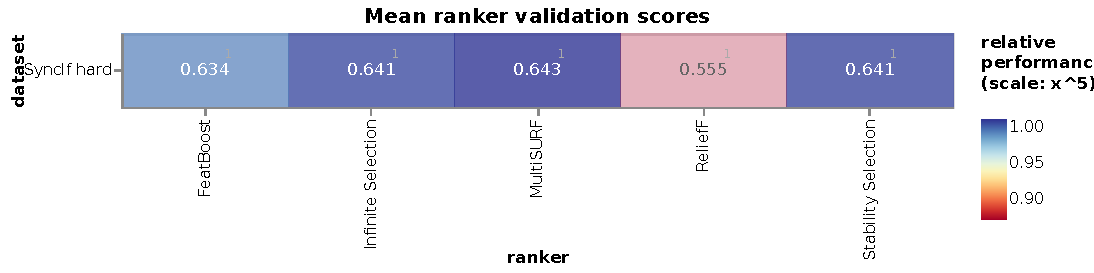
\includegraphics[width=\linewidth]{report/images/results-validation-with-mean-score-tabular.pdf}
    \caption{Mean \gls{dt} validation scores plotted with emphasized \textbf{relative performance}. The \textit{relative performance} is a ranker's mean validation score as a fraction of the highest achieved score by any ranker for some dataset. Same curves as in Figure~\ref{fig:results-validation-dt-various-rankers} and Figure~\ref{fig:results-validation-with-mean-score}.}
    \label{fig:results-validation-with-mean-score-tabular}
\end{figure}
% \todo{add relative performance calculation in theoretical section}

This time (Figure~\ref{fig:results-validation-with-mean-score-tabular}), the summarized performance of each feature ranker is visible in an instant. The coloring of the chart adjusts according to the \textbf{relative performance} of the ranker, with respect to the best performing ranker. This is computed simply by taking the ranker's mean validation score as a fraction of the highest score achieved by any ranker. This means that a relative performance of $1.00$ resembles the highest performing ranker, and a relative performance of $0.50$ would mean a ranker gets only half of the highest performing ranker's score. An accompanying color scale illustrates this fact, where blue resembles a higher score and red a lower score. Furthermore, the differences are further exacerbated by use of an \textit{exponential} color scale. In this case, an exponent of $x^5$ is chosen, to be able to better differentiate between the top performers. The best score also gets its font weight displayed as \textit{bold}, such to emphasize the best performing ranker.
It is thereby important to note that in case \textit{multiple} datasets are considered, each dataset gets its own relative performance scale. This is because the scores across multiple datasets ought not to be compared directly to each other.



% R2- and Log loss scores
Again the R\textsuperscript{2}- and log loss scores are investigated, which are computed using the ground-truth relevant features. The hypothesis is that the scores are able to `predict' the validation estimator's performance. This is useful because, by evaluating the quality of the feature ranking directly, one could already make meaningful conclusions, just by having run the ranker alone. A comparison chart for these metrics is plotted in Figure~\ref{fig:results-ground-truth-various-rankers}.

\begin{figure}[ht]
     \centering
     \begin{subfigure}[b]{0.49\textwidth}
        \centering
        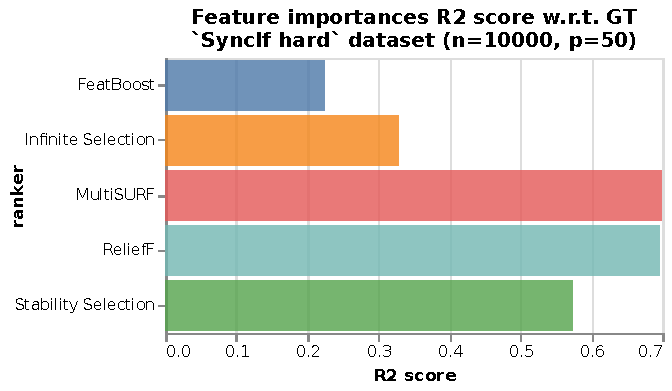
\includegraphics[width=\linewidth]{report/images/results-r2-score-various-rankers.pdf}
        \caption{The average R\textsuperscript{2} score over all bootstraps. A \textbf{higher} score is better. Computed like explained in Section~\ref{section:feature-importance-definition}.}
        \label{fig:results-r2-score-various-rankers}
     \end{subfigure}
     \hfill
     \begin{subfigure}[b]{0.49\textwidth}
        \centering
        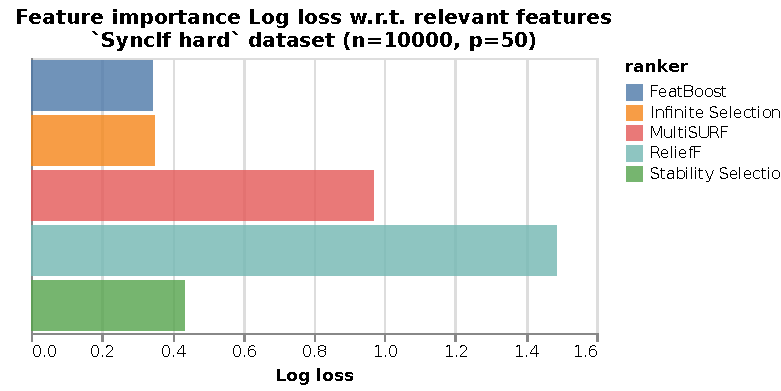
\includegraphics[width=\linewidth]{report/images/results-log-loss-various-rankers.pdf}
        \caption{The average log-loss score over all bootstraps. \textbf{Lower} is better. Computed like explained in Section~\ref{section:feature-importance-definition}.}
        \label{fig:results-log-loss-various-rankers}
     \end{subfigure}
     
    \caption{Log loss and R\textsuperscript{2} scores, computed by comparing the \textit{estimated} feature importance scores against the feature importance \textit{ground-truth}. Such a ground-truth is available when datasets are synthetically generated. Scores shown for `Synclf hard' dataset on multiple rankers.}
    \label{fig:results-ground-truth-various-rankers}
\end{figure}

For Figure~\ref{fig:results-ground-truth-various-rankers} it is, first of all, important to note that the R\textsuperscript{2}- and log loss scores were computed as an average score over all bootstraps. This means that after running a single ranker on a single dataset, $B$ such scores are obtained - which are then aggregated into a single score by taking its mean. In the figure it can be seen, that in the case of the R\textsuperscript{2} score the scorings represent the scores presented in Figure~\ref{fig:results-validation-with-mean-score} and Figure~\ref{fig:results-validation-with-mean-score-tabular} very well. The order of best performance w.r.t. mean validation score was predicted by the R\textsuperscript{2} score: wherever the R\textsuperscript{2} score is higher, the mean validation performance is also higher. The same applies to the log loss scores: more loss means worse mean validation performance. Although in this example the differences are very small, still a measure of proportionality between the scores exists, for this dataset.


To assess the \textbf{stability} of the rankers, the feature importances of the various rankers can be put side-by-side. Then, the standard deviations of each feature estimated over $B$ bootstraps can be shown. This can be seen illustrated in Figure~\ref{fig:results-importances-stability-multiple-rankers}.

\begin{figure}[ht]
    \centering
    % 800x190
    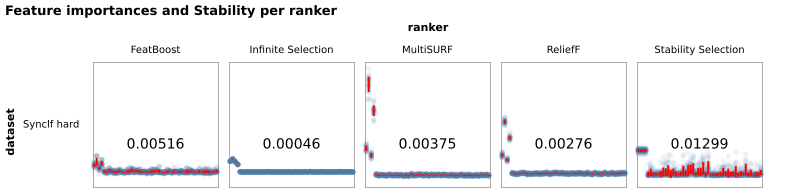
\includegraphics[width=\linewidth]{report/images/results-importances-stability-multiple-rankers.png}
    \caption{The estimated feature importances and their stabilities, quantified using the mean standard deviation over all feature importances. Plots shown for `Synclf hard' dataset.}
    \label{fig:results-importances-stability-multiple-rankers}
\end{figure}

As can be seen in Figure~\ref{fig:results-importances-stability-multiple-rankers}, the stability of the ranking algorithms varies. As illustrated by the red standard deviation error bars, the algorithms have varying amounts of deviation in their feature importance estimations. Whereas Infinite Selection is very stable, and shows hardly any variance over the bootstraps at all, Stability Selection is very unstable, despite its name. MultiSURF can be seen to be varying mainly in the relevant features, similarly to ReliefF. Looking at the summarized stability value, indeed the expected instabilities are captured in the scalar. Stability Selection has the highest mean standard deviation and Infinite Selection has the lowest. This indicates the metric might be successful in capturing the instability of the algorithms.


% next section
Now that all relevant plots are clarified and understood, a broader view can be taken. In the next section, the experiment in its entirety will be considered.



%%% ALL RESULTS %%
\subsection{Experimental result for all datasets}
Now, a look is taken at the results of \textit{all} datasets. See Figure~\ref{fig:results-all-datasets-mean-validation-dt}, which is explained below.

\begin{figure}[ht]
    \centering
    % 1000x400
    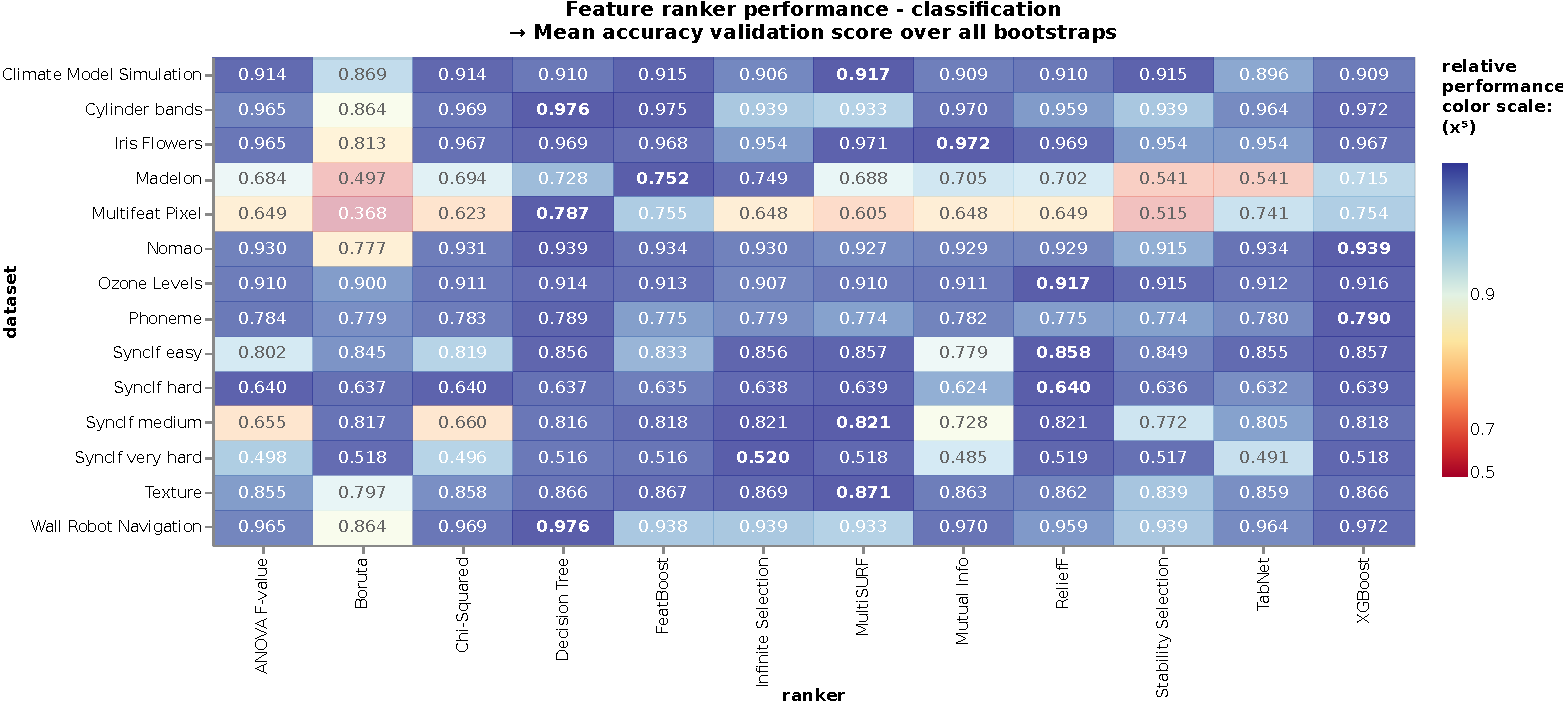
\includegraphics[width=\linewidth]{report/images/results-all-datasets-mean-validation-dt.pdf}
    \caption{Mean \textbf{classification} accuracy validation scores for all datasets and all rankers. Color scale is configured with \textit{relative performance}, like explained in Section~\ref{section:experiments-example}. Validation scores shown are for classification datasets using a \gls{dt} as a validator.}
    \label{fig:results-all-datasets-mean-validation-dt}
\end{figure}

To illustrate the performance of the complete experiment, different ways of visualization are required. With this many combinations of feature rankers and datasets, no longer can the line curves showing the mean validation scores be used to explain the findings. Instead, it is chosen to display this data in a heatmap, exactly similar to Figure~\ref{fig:results-validation-with-mean-score-tabular}, but with more data. Various aspects of performance are discussed, starting with the \textbf{mean validation} performance. 



In Figure~\ref{fig:results-all-datasets-mean-validation-dt} it can be seen that the table coloring reveals much about the performance of the feature ranker. The more the coloring is toward dark \textit{blue}, the better the ranker performed. On the other hand, red indicates bad performance: the worst case in this plot is Boruta, which only achieves about half the score of the best performer for the `Multifeat Pixel' dataset. Boruta's bad performance is almost certainly due to a configuration anomaly, since the performance is worse than random in some cases. A notable performer is the \textbf{\gls{dt}}, used as a Feature Ranker by making use of its computed feature importance scores. The algorithm scores high on nearly every dataset, making it a good contender for the best performer. It might seem odd, however, that a \gls{dt} is run for Feature Selection first, and then \textit{also} for validation. For this reason, the experiment was also run with another validation estimator, \gls{knn}. For this, see Figure~\ref{fig:results-all-datasets-mean-validation-knn} in the Appendix.

Next is the algorithm \textbf{stability}. The algorithm stability scores were computed like illustrated in the previous section, but now for more datasets. The scores were represented in a table and have a custom color scheme applied to it to better emphasize the differences. See Figure~\ref{fig:results-all-datasets-stability-scores}.

\begin{figure}[ht]
    \centering
    % 1000x450
    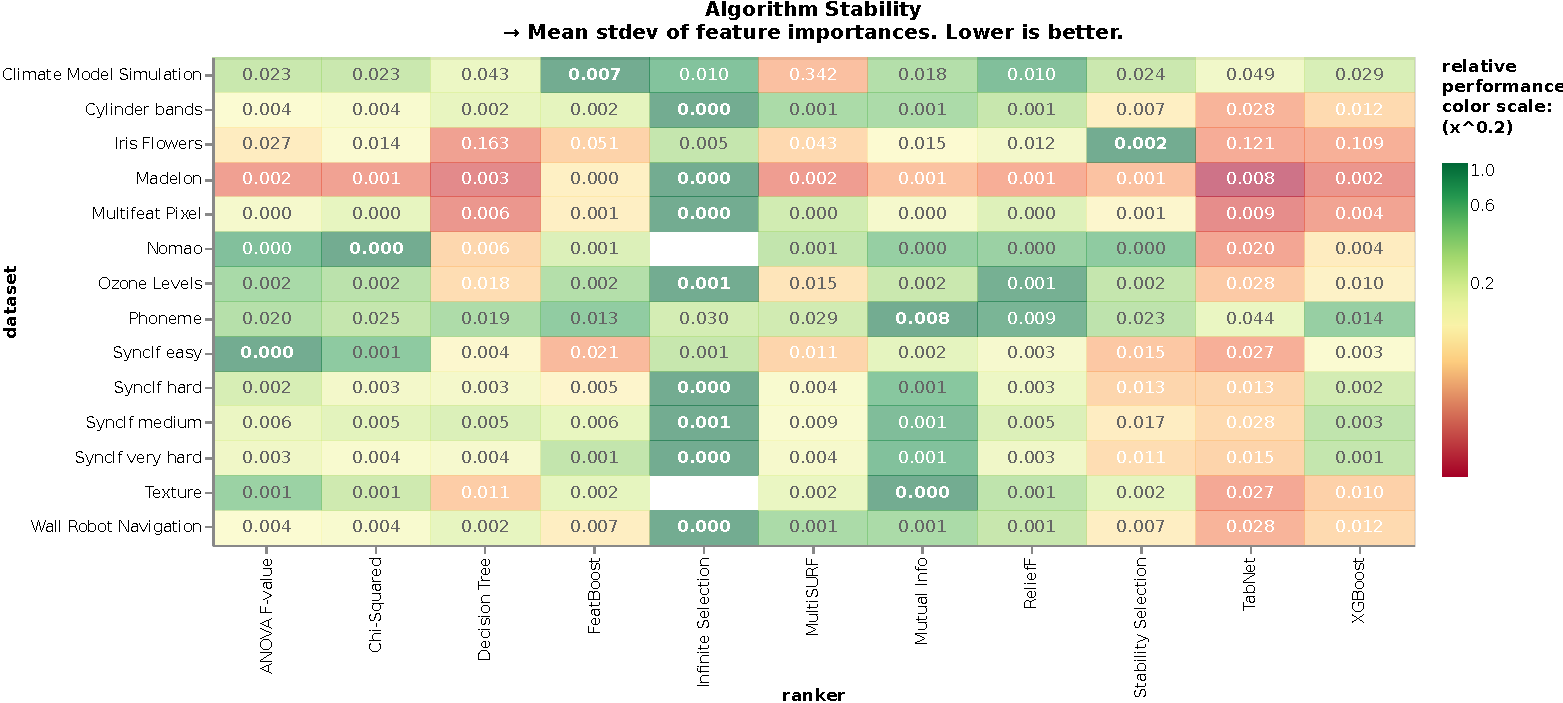
\includegraphics[width=\linewidth]{report/images/results-all-datasets-stability-scores.pdf}
    \caption{Algorithm stability scores. Obtained by computing the standard deviation over the feature importance vectors, like illustrated in Section~\ref{section:experiments-example} and explained in Section~\ref{section:feature-importance-stability}. A custom color scheme was chosen to better emphasize the differences. A darker shade of red means worse stability. A darker shade of green means better stability. The empty cells are due to an experiment failure.}
    \label{fig:results-all-datasets-stability-scores}
\end{figure}

Like can be seen in Figure~\ref{fig:results-all-datasets-stability-scores}, the stability scores differ per ranker. Especially TabNet, XGBoost and Decision Tree can be seen to be relatively unstable. Infinite Selection, Mutual Info and ReliefF, on the other hand, have a better stability.

Next, a look is taken at the computed R\textsuperscript{2} scores. The scores were computed using the \gls{apriori} known relevant features, i.e., the datasets \gls{gt} feature importances. A comparison heatmap plot can be seen in Figure~\ref{fig:results-all-datasets-r2-scores}.

\begin{figure}[ht]
    \centering
    % 800x250
    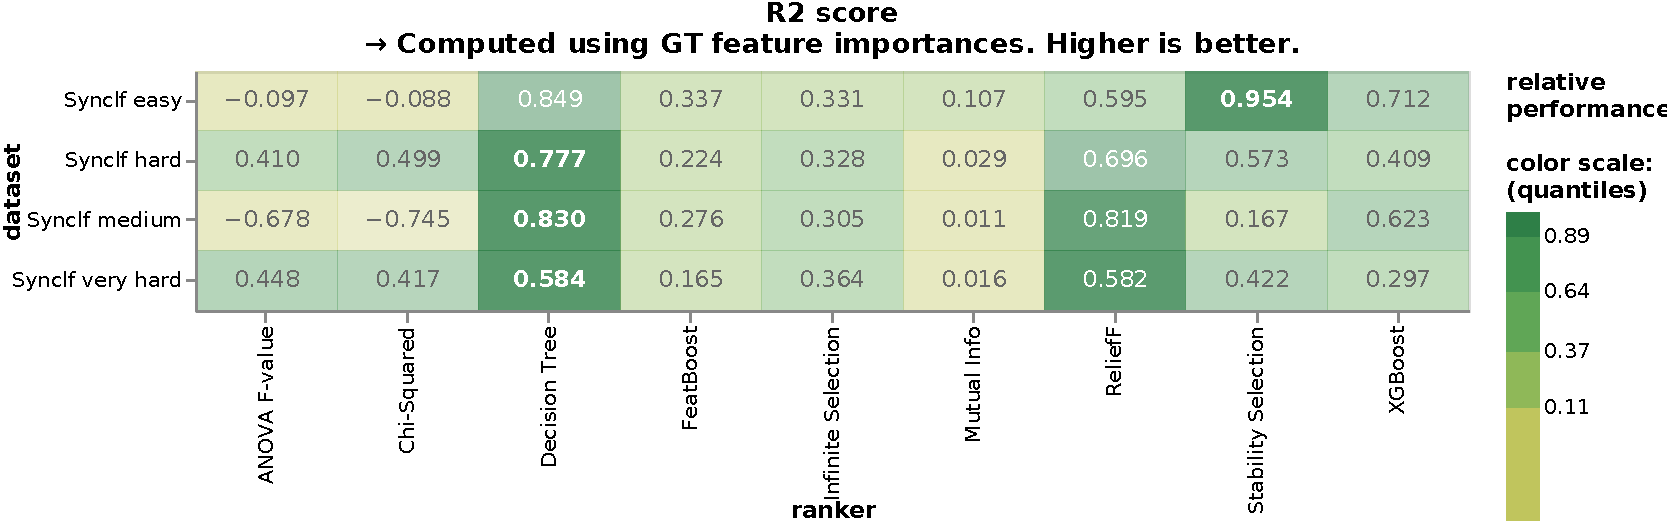
\includegraphics[width=\linewidth]{report/images/results-all-datasets-r2-scores.pdf}
    \caption{Algorithm R\textsuperscript{2} scores, computed using the \gls{gt} feature importanes. The computation was explained in Section~\ref{section:evaluation-apriori-knowledge} and illustrated in Section~\ref{section:experiments-example}. A darker shade of green means a better score.}
    \label{fig:results-all-datasets-r2-scores}
\end{figure}

As could be seen in Figure~\ref{fig:results-all-datasets-r2-scores}, the differences in R\textsuperscript{2} scores are notable, and correlate slightly with the mean validation scores for the designated datasets. Both \gls{dt} and ReliefF have high R\textsuperscript{2} scores for the chosen datasets. FeatBoost, however, had a high overall mean validation score but cannot be seen to have a high R\textsuperscript{2} score. This might indicate that the scoring does not always foretell validation performance.

Especially in the case of FeatBoost and Infinite Selection, there exist big discrepancies between the mean validation score and the computed R\textsuperscript{2} scores. Whereas for both rankers the mean validation scores are high for the `Synclf' datasets, the R\textsuperscript{2} scores did not follow. A reason for this might be the fact that these rankers do often rank features as having an importance of above zero. Whereas an algorithm might still get the feature importance \textit{order} correct, the algorithm does a worse job in the R\textsuperscript{2} scoring due to always giving features scores of well above zero. Other rankers, that assign more importance to some presumably relevant features but less to the others, will be better off with the R\textsuperscript{2} scoring. The metric might therefore pose an unfair advantage to how rankers behave in this regard.

In a similar fashion, the log loss scores are plotted. See Figure~\ref{fig:results-all-datasets-log-loss}.

\begin{figure}[ht]
    \centering
    % 800x250
    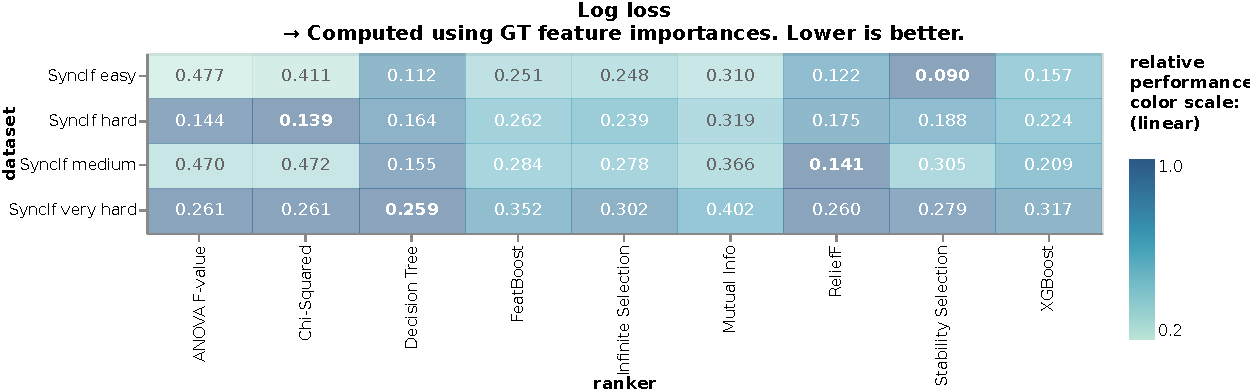
\includegraphics[width=\linewidth]{report/images/results-all-datasets-log-loss.pdf}
    \caption{Algorithm Log loss scores, computed using the \gls{gt} feature importanes. The computation was explained in Section~\ref{section:evaluation-apriori-knowledge} and illustrated in Section~\ref{section:experiments-example}. A darker shade of blue means a better score.}
    \label{fig:results-all-datasets-log-loss}
\end{figure}

In the case of the log loss metric, a different pattern is visible (Figure~\ref{fig:results-all-datasets-log-loss}). Indeed, well performing rankers are \gls{dt} and ReliefF. The scoring did miss FeatBoost and Infinite Selection, however, as being overall good performers. Whereas according to the \textit{mean} validation scores FeatBoost and Infinite Selection are among the top performers, this is not reflected in the log loss score. This might, again, be due to an unfair advantage given to rankers that tend to score irrelevant features closer to zero. This is similar to the R\textsuperscript{2} score, though arguably the effect is exaggerated in the case of the R\textsuperscript{2} score. The metrics might therefore not be ideal for direct algorithm comparison: it is best the mean validation scores are included at all times. The metrics can, however, reveal interesting information in specific scenarios. This might be the case, for example, when no feature selection is applied at all in the evaluation process, and all one has is the feature importance ground truth and estimations.

Additionally, some plots can be seen in the Appendix. A plot showing the validation scores using \gls{knn} as the validation estimator can be found in the Appendix Figure~\ref{fig:results-all-datasets-mean-validation-knn}. To see the R\textsuperscript{2} scores and Log loss scores for the \textit{regression} datasets, see Figure~\ref{fig:results-all-datasets-log-loss-regression} and Figure~\ref{fig:results-all-datasets-r2-score-regression}, respectively. The regression dataset mean validation scores can be seen in Figure~\ref{fig:results-all-datasets-mean-validation-dt-regression}.


\subsection{Learning curves and time complexity}
To first get an idea of the algorithm time complexity, an overview plot is taken into consideration. In this plot, multiple datasets and multiple rankers are considered. For each benchmark, the fitting time in seconds is plotted. See Figure~\ref{fig:results-all-datasets-fitting-time}.

\begin{figure}[ht]
    \centering
    % 1000x300
    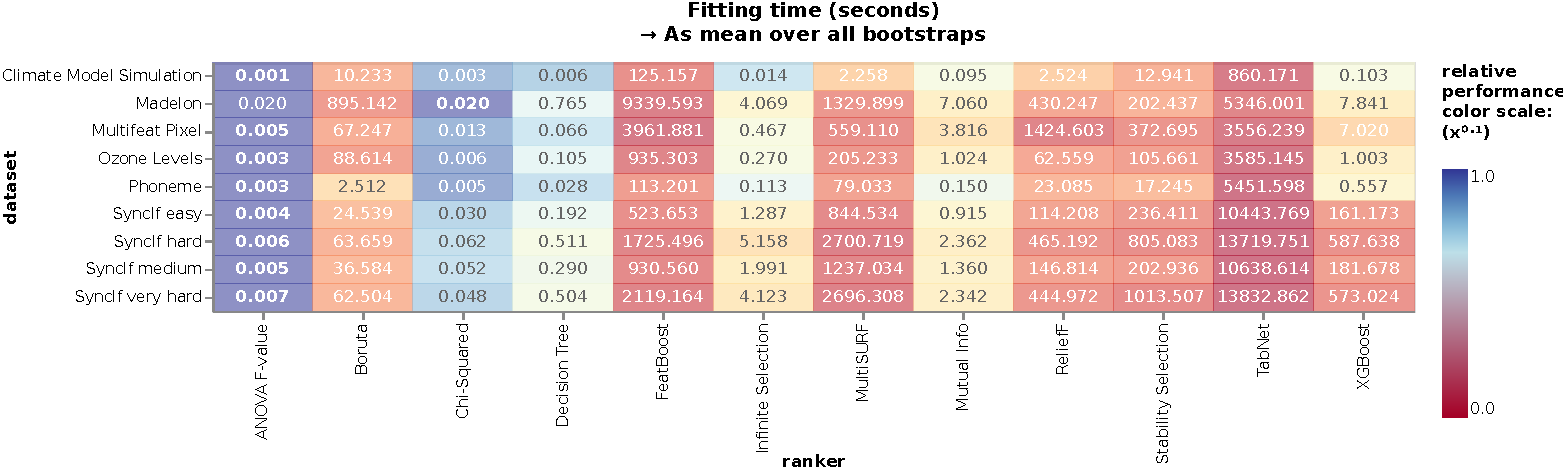
\includegraphics[width=\linewidth]{report/images/results-all-datasets-fitting-time.pdf}
    \caption{Mean fitting times from running the experiment $B=25$ times. Fitting times are represented in seconds. A custom color scheme and scaling factor was chosen to emphasize the differences in fitting times.}
    \label{fig:results-all-datasets-fitting-time}
\end{figure}


In Figure~\ref{fig:results-all-datasets-fitting-time} it can first of all be seen that the algorithms differ immensely in fitting times. TabNet is (by far) the most complex and time-consuming estimator to fit. This is much due to the fact that it fits a sophisticated Neural Network and uses PyTorch to do so. The two algorithms that are next in time complexity are MultiSURF and FeatBoost. Some statistical estimators can be seen to have very low fitting times.

To investigate algorithm performance under varying conditions of \textbf{sample size}, a separate experiment was run. In this experiment, only the `Synclf hard' dataset is considered. Then, the sample size for this dataset was varied over a number of intervals, set to a fixed number each time. The sample size was set to range from 100 to 2,100 with intervals of 200. Note, that the total sample size for this dataset is 10,000. For every sample size, 10 bootstraps were run.

In this way, two things can be investigated. (1) the time complexity and (2) the learning curve behavior of the various algorithms. Both were plotted. First, a look is taken at the time complexity. To investigate the time complexity of the algorithms, the fitting time was recorded. The fitting time was measured to entail only exactly the ranker fitting step - no supplementary preprocessing steps whatsoever influenced the time recording. The time was stored in a high-accuracy float but represented as \textit{seconds}.  See Figure~\ref{fig:results-time-complexity}.

\begin{figure}[ht]
    \centering
    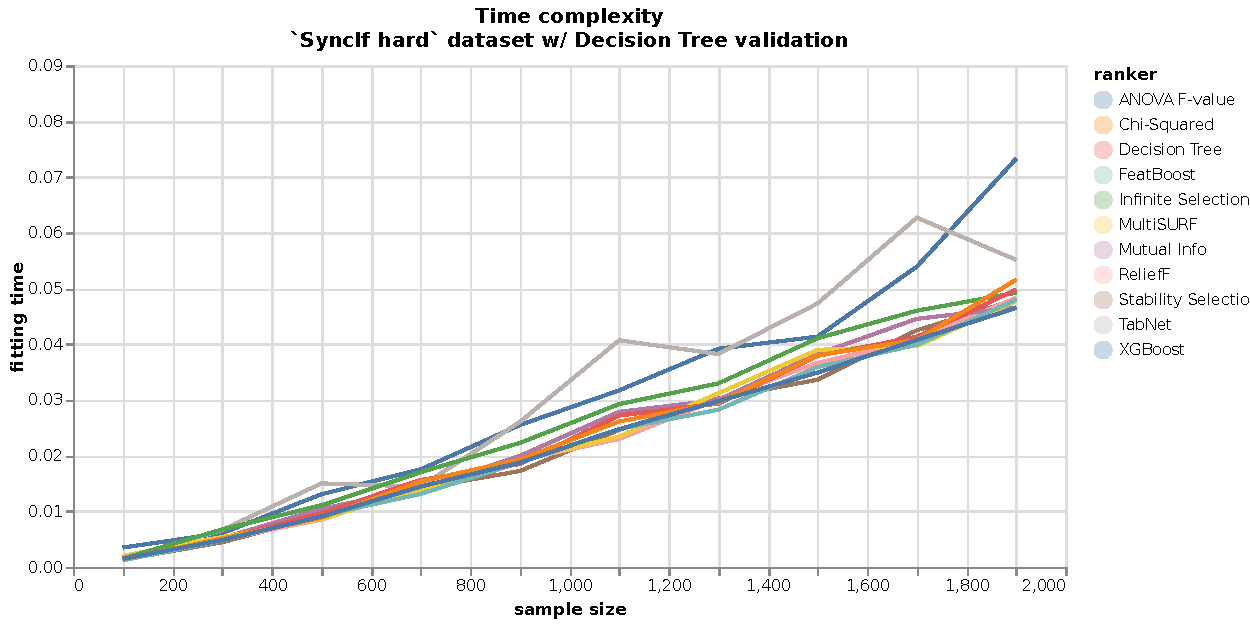
\includegraphics[width=\linewidth]{report/images/results-time-complexity.pdf}
    \caption{Time complexity plot for `Synclf hard' dataset. Sample sizes from 100 to 2,100 were used, with intervals of 200. The plot shows the average fitting time over 10 bootstraps.}
    \label{fig:results-time-complexity}
\end{figure}

As can be seen in Figure~\ref{fig:results-time-complexity}, most algorithms scale about slightly worse than linear when increasing the number of samples. It can be seen that when 1,000 samples are used versus 2,000, the fitting time is about double. The only outliers are XGBoost and TabNet, which seem to need a bit longer than its competitors when the sample size exceeds 900.

The learning curve was omitted from the main text and can be seen in the Appendix. See Figure~\ref{fig:results-learning-curve}. It can be seen that the algorithms learn very similarly given an increasing number of available samples. Only stability selection and mutual info are having a slightly harder time learning the useful features with little data.

\subsection{Online dashboard}
In case the reader is interested in exploring the data interactively him- or herself, the plots above can also be accessed on the online dashboard\footnote{\href{https://wandb.ai/dunnkers/fseval/reports/Final-results-MSc-Thesis--Vmlldzo3ODEyODE}{https://wandb.ai/dunnkers/fseval/reports/Final-results-MSc-Thesis--Vmlldzo3ODEyODE}}. The dashboard lets the user see the data in more detail by the use of zooming and tooltips. Moreover, the visualizations contain hyperlinks, taking the user directly to a detailed page of a single benchmark run.

\biblio
\end{document}
